\documentclass[a4paper,12pt]{book}
\usepackage[utf8]{inputenc}
\title{}
\author{Rachel Morris}
\date{\today}

\usepackage{rachwidgets}
\usepackage{fancyhdr}
\usepackage{lastpage}
\usepackage{dirtree}
\usepackage{boxedminipage}

\newcommand{\laClass}{CS 211\ }
\newcommand{\laSemester}{Fall 2017\ }
\newcommand{\laChName}{Connections to Matrices and Relations\ }
\newcounter{question}

\setcounter{chapter}{7}
\setcounter{section}{3}
\newcommand{\laChapter}{7.4 \laChName}

\pagestyle{fancy}
\fancyhf{}
\lhead{\laClass Exercise, \laSemester}
\chead{}
\rhead{Ch \laChapter}
\rfoot{\thepage\ of \pageref{LastPage}}
\lfoot{\scriptsize Compiled by Rachel Morris, last updated \today}

\renewcommand{\headrulewidth}{2pt}
\renewcommand{\footrulewidth}{1pt}

\begin{document}

    %\toggletrue{answerkey}
    \togglefalse{answerkey}

    \section{\laChName}
    
    \notonkey{

    %- Team Info ------------------------------------------------------%

    Please write down all people in your team. ~\\

    % table %
    \begin{tabular}{ p{6cm} p{6cm} }
        1. & 2. \\ \\
        3. & 4.
    \end{tabular} ~\\
    % table %
    
    \hrulefill
    
    }{}


    \subsection{Adjacency matrix}

    \notonkey{

        \begin{introNOHEAD}{}
            Given a graph $G$ with vertex set $V = \{ v_{1}, v_{2}, ..., v_{n} \}$
            and edge set $E$, we define the \textbf{adjacency matrix} of $G$ as
            follows. The matrix $M$ is an $n \times n$ array of natural numbers,
            which we imagine having rows and columns labelled as follows:

            \begin{center}
                \begin{tikzpicture}
                    \node[left] at (0,4) {Row $1 \to$};
                    \node[left] at (0,3) {Row $2 \to$};
                    \node[left] at (0,2) {Row $3 \to$};
                    \node[left] at (0,1) {Row $...$};
                    \node[left] at (0,0) {Row $n \to$};
                    \node[above] at (3,4.5) {Columns $1, 2, ..., n$};
                    \draw (0.5,0) -- (0,0) -- (0,4) -- (0.5,4);
                    \draw (5.5,0) -- (6,0) -- (6,4) -- (5.5,4);
                \end{tikzpicture}
            \end{center}


            The entry in row $i$, column $j$ (referred to as the $(i,j)$ - entry of $M$ or,
            more concisely, $M_{ij}$) is defined as

            \begin{center}
                $M_{ij} = $ the number of edges connecting $v_{i}$ and $v_{j}$ in $G$.
            \end{center}
            \footnote{Discrete Mathematics, by Ensley and Crawley}
        \end{introNOHEAD}

    }{}

\notonkey{ \newpage }{ \hrulefill }

% -------------------------------------------------------------%
% - QUESTION --------------------------------------------------%
% -------------------------------------------------------------%
\stepcounter{question}
\begin{question}{\thequestion}{2}
    % Page 547

    Fill out the adjacency matrix for the following graph.
    ~\\
    \begin{center}
        
        \begin{tikzpicture}
            \filldraw (-7,1) circle (1pt) node[left] {1};
            \filldraw (-7,2) circle (1pt) node[left] {2};
            \filldraw (-6,3) circle (1pt) node[above] {3};
            \filldraw (-5,1) circle (1pt) node[right] {5};
            \filldraw (-5,2) circle (1pt) node[right] {4};

            \draw (-7,1) -- (-5,1);
            \draw (-7,1) -- (-7,2);
            \draw (-7,2) -- (-5,2);
            \draw (-7,2) -- (-6,3);
            \draw (-7,1) to[bend right] (-5,1);
            \draw (-4.7,2) circle (10pt);
            
            \node[above,rotate=90] at (-0.5, 2) {Rows};
            \node[left] at (0,4) {1};
            \node[left] at (0,3) {2};
            \node[left] at (0,2) {3};
            \node[left] at (0,1) {4};
            \node[left] at (0,0) {5};
            \node[above] at (3,5) {Columns};
            \node[above] at (1,4.5) {1};
            \node[above] at (2,4.5) {2};
            \node[above] at (3,4.5) {3};
            \node[above] at (4,4.5) {4};
            \node[above] at (5,4.5) {5};
            \draw (0.5,-0.5) -- (0,-0.5) -- (0,4.5) -- (0.5,4.5);
            \draw (5.5,-0.5) -- (6,-0.5) -- (6,4.5) -- (5.5,4.5);

            \solution{ \node at (1,0) {2}; }{}
            \solution{ \node at (2,0) {0}; }{}
            \solution{ \node at (3,0) {0}; }{}
            \solution{ \node at (4,0) {0}; }{}
            \solution{ \node at (5,0) {0}; }{}
            
            \solution{ \node at (1,1) {0}; }{}
            \solution{ \node at (2,1) {1}; }{}
            \solution{ \node at (3,1) {0}; }{}
            \solution{ \node at (4,1) {1}; }{}
            \solution{ \node at (5,1) {0}; }{}
            
            \solution{ \node at (1,2) {0}; }{}
            \solution{ \node at (2,2) {1}; }{}
            \solution{ \node at (3,2) {0}; }{}
            \solution{ \node at (4,2) {0}; }{}
            \solution{ \node at (5,2) {0}; }{}
            
            \solution{ \node at (1,3) {1}; }{}
            \solution{ \node at (2,3) {0}; }{}
            \solution{ \node at (3,3) {1}; }{}
            \solution{ \node at (4,3) {1}; }{}
            \solution{ \node at (5,3) {0}; }{}
            
            \solution{ \node at (1,4) {0}; }{}
            \solution{ \node at (2,4) {1}; }{}
            \solution{ \node at (3,4) {0}; }{}
            \solution{ \node at (4,4) {0}; }{}
            \solution{ \node at (5,4) {2}; }{}
        \end{tikzpicture}
    \end{center}
    
\end{question}

\hrulefill

% -------------------------------------------------------------%
% - QUESTION --------------------------------------------------%
% -------------------------------------------------------------%
\stepcounter{question}
\begin{question}{\thequestion}{2}
    
    Draw a graph that corresponds to the adjacency matrix.
    This is a directed graph, so the matrix is not symmetric.
    It should be read as row $i$ $\to$ column $j$. For example,
    row 1 shows that it goes from $1 \to 2$, $1 \to 4$, and $1 \to 5$.
    % Exercise 1

    ~\\
        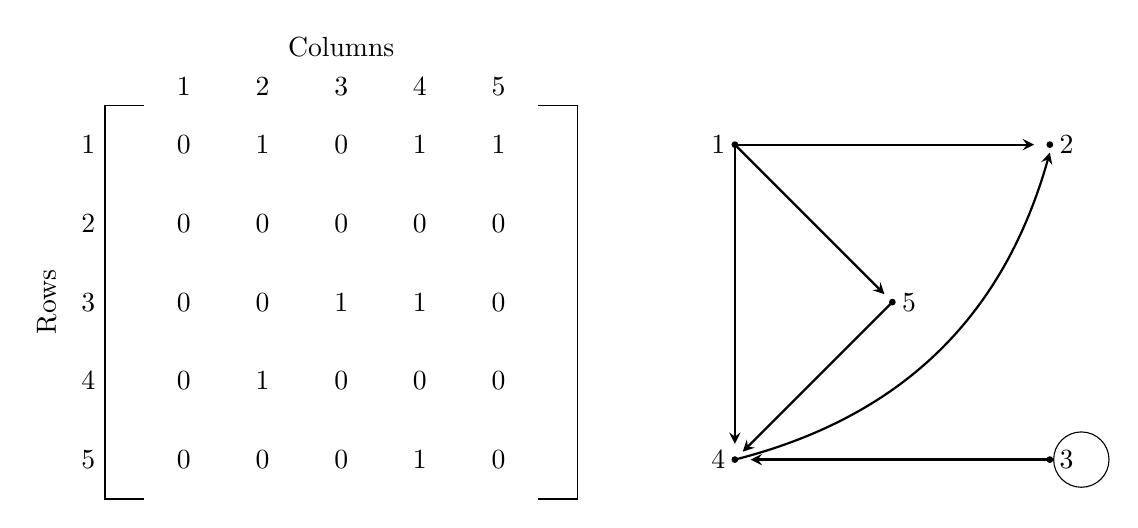
\begin{tikzpicture}[arrow/.style = {thick,-stealth}]
            \node[above,rotate=90] at (-0.5, 2) {Rows};
            \node[left] at (0,4) {1};
            \node[left] at (0,3) {2};
            \node[left] at (0,2) {3};
            \node[left] at (0,1) {4};
            \node[left] at (0,0) {5};
            \node[above] at (3,5) {Columns};
            \node[above] at (1,4.5) {1};
            \node[above] at (2,4.5) {2};
            \node[above] at (3,4.5) {3};
            \node[above] at (4,4.5) {4};
            \node[above] at (5,4.5) {5};
            \draw (0.5,-0.5) -- (0,-0.5) -- (0,4.5) -- (0.5,4.5);
            \draw (5.5,-0.5) -- (6,-0.5) -- (6,4.5) -- (5.5,4.5);

            \node at (1,0) {0};
            \node at (2,0) {0};
            \node at (3,0) {0};
            \node at (4,0) {1};
            \node at (5,0) {0};
            
            \node at (1,1) {0};
            \node at (2,1) {1};
            \node at (3,1) {0};
            \node at (4,1) {0};
            \node at (5,1) {0};
            
            \node at (1,2) {0};
            \node at (2,2) {0};
            \node at (3,2) {1};
            \node at (4,2) {1};
            \node at (5,2) {0};
            
            \node at (1,3) {0};
            \node at (2,3) {0};
            \node at (3,3) {0};
            \node at (4,3) {0};
            \node at (5,3) {0};
            
            \node at (1,4) {0};
            \node at (2,4) {1};
            \node at (3,4) {0};
            \node at (4,4) {1};
            \node at (5,4) {1};

            \solution{
                \filldraw (8, 0)  circle (1pt) node[left]    {4};
                \filldraw (12,0)  circle (1pt) node[right]   {3};
                \filldraw (8, 4)  circle (1pt) node[left]    {1};
                \filldraw (12,4)  circle (1pt) node[right]   {2};
                \filldraw (10,2)  circle (1pt) node[right]   {5};

                \draw[arrow] (8,4)  -- (8,0.2);
                \draw[arrow] (8,4)  -- (9.9, 2.1);
                \draw[arrow] (10,2) -- (8.1,0.1);
                \draw[arrow] (8,4)  -- (11.8,4);
                \draw[arrow] (12,0) -- (8.2,0);
                \draw (12.4,0) circle (10pt);
                \draw[arrow] (8,0) to[bend right] (12,3.9);
            }{}
        \end{tikzpicture}
    
\end{question}

\notonkey{ \newpage }{ \hrulefill }

    \subsection{Directed graphs}

    \begin{introNOHEAD}{}
        \begin{enumerate}
            \item   A \textbf{directed graph}, like a graph, consists of
                    a set $V$ of vertices and a set $E$ of edges.
                    Each edge is associated with an ordered pair of
                    vertices called its \textbf{endpoints}.
                    In other words, a directed graph is the same as a graph,
                    but the edges are described as \textit{ordered pairs}
                    rather than unordered pairs;

            \item   If the endpoints for edge $e$ are $a$ and $b$ in that order,
                    we say $e$ is an edge \textbf{from $a$ to $b$}, and
                    in the diagram we draw the edge as a straight or curved
                    arrow from $a$ to $b$.

            \item   For a directed graph, we use $(a,b)$ rather than
                    [$a$, $b$] to indicate an edge from $a$ to $b$.
                    This emphasizes that the edge is an \textbf{ordered pair},
                    by utilizing the usual notation for ordered pairs.

            \item   A \textbf{walk} in a directed graph in a sequence
                    $v_{1}e_{1} v_{2}e_{2} ... v_{n}e_{n} v_{n+1}$
                    of alternating vertices and edges that begins and
                    ends with a vertex, and where each edge in the
                    list between its endpoints in the proper order.
                    (That is, $e_{1}$ is an edge from $v_{1}$ to $v_{2}$,
                    $e_{2}$ is an edge from $v_{2}$ to $v_{3}$, and so on.)
                    If there is no chance of confusion, we omit the
                    edges when we describe a walk.

            \item   The \textbf{adjacency matrix} for a directed graph
                    with vertices \\ $\{ v_{1}, v_{2}, ..., v_{n} \}$ is
                    the $n \times n$ matrix where $M_{ij}$ (the entry
                    in row $i$, column $j$) is the number of edges
                    from vertex $v_{i}$ to vertex $v_{j}$.
        \end{enumerate}
        \footnote{Discrete Mathematics, Ensley and Crawley}
    \end{introNOHEAD}


% -------------------------------------------------------------%
% - QUESTION --------------------------------------------------%
% -------------------------------------------------------------%
\stepcounter{question}
\begin{question}{\thequestion}{2}


    Draw a directed graph with vertices $V = \{ 1, 2, 3, 4, 5 \}$ and edges
    \\ $E = \{ (1,4), (1,5), (2,1), (3,4), (4,3), (5,2) \}$.

    \solution{
    
        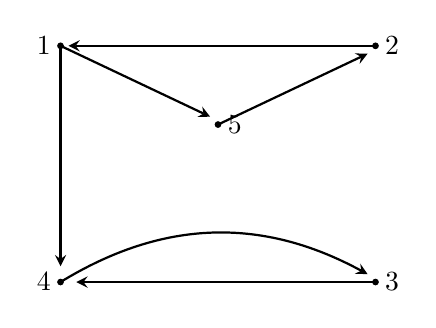
\begin{tikzpicture}[arrow/.style = {thick,-stealth}]
            \filldraw (8, 0)  circle (1pt) node[left]    {4};
            \filldraw (12,0)  circle (1pt) node[right]   {3};
            \filldraw (8, 3)  circle (1pt) node[left]    {1};
            \filldraw (12,3)  circle (1pt) node[right]   {2};
            \filldraw (10,2)  circle (1pt) node[right]   {5};

            \draw[arrow] (8,3)  -- (8,0.2);
            \draw[arrow] (8,3)  -- (9.9, 2.1);
            \draw[arrow] (10,2) -- (11.9,2.9);
            \draw[arrow] (12,3)  -- (8.1,3);
            \draw[arrow] (12,0) -- (8.2,0);
            \draw[arrow] (8,0) to[bend left] (11.9,0.1);
        \end{tikzpicture}
        
    }{}
    
\end{question}
















\end{document}
